\chapter{Implementierung}
\label{chap:implementierung}

Die Implementierung stützt sich auf die in \ref{sec:ziele} definierten Entwicklungsziele. Zuerst soll auf die Projektstruktur und das Assembling eingegangen werden. Danach wird die Integration verschiedener APIs und die eigentliche Anwendungs-Architektur besprochen. 


\section{Projektstruktur und Assembling}
\label{sec:struktur}

Die Anwendung wird in zwei grundlegende Module gegliedert. Diese bilden das Back-End und Front-End und sind anhand Graphik  \\

\begin{figure}[H]
  \centering  
  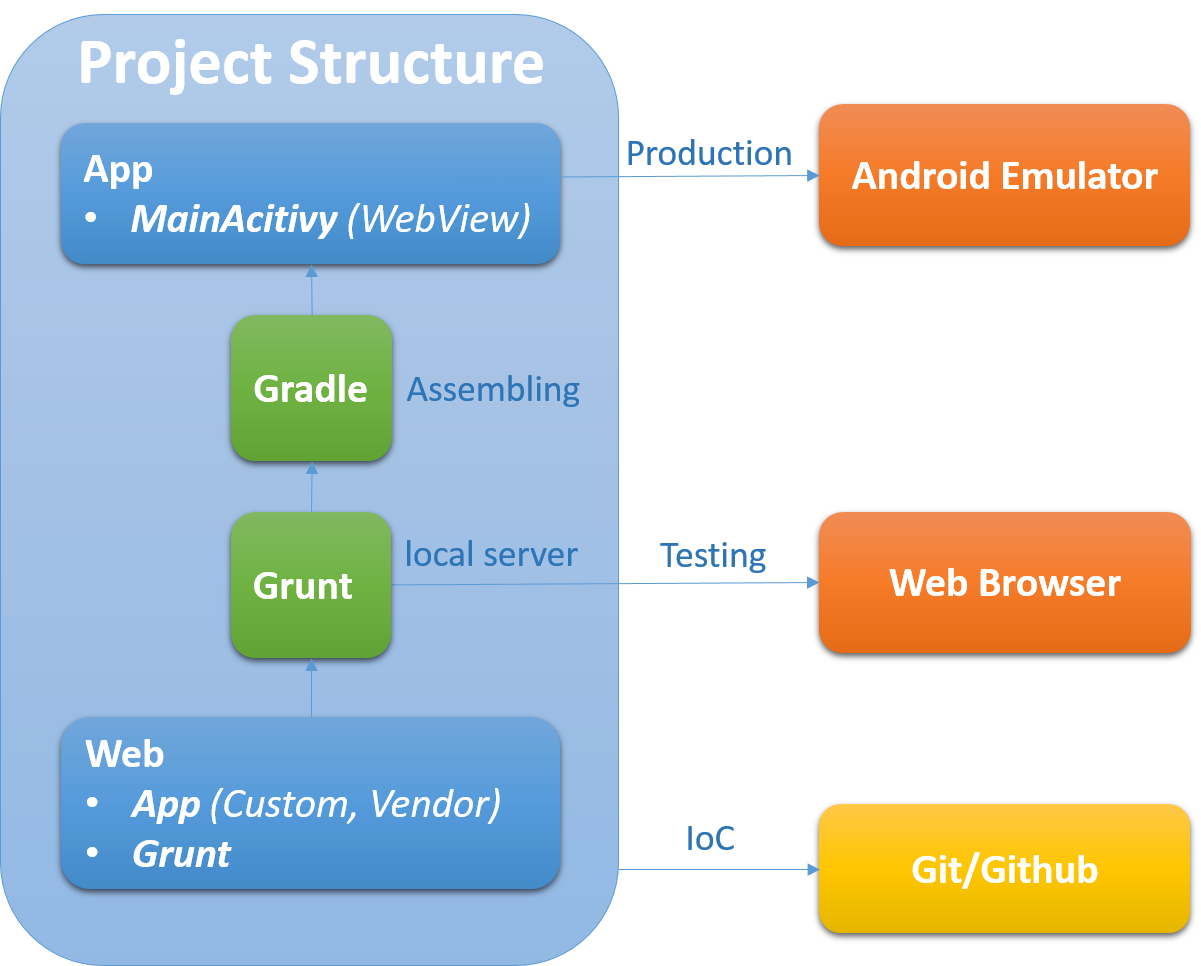
\includegraphics[scale=0.5]{img/project.png}
  \caption{Sighted! - Projektstruktur}
  \label{fig:mapping}
\end{figure}

Das erste Modul 'App' bildet das Back-End. Dieses startet das Hauptprogramm mittels der Java-Klasse MainActitivy. Dort wird der Webview initialisiert und verschiedene hardwarenahe Konfigurationen getroffen. Zu diesen Konfigurationen zählen beispielsweise bereitgestellt Rechte, die die Steuerung der Anwendung durch Javascript betreffen. \\
Das zweite Modul 'Web' bildet das Front-End. Dort werden alle Inhalte des Web-Projekts gespeichert, wie Anwendungslogik und verschiedene Javascript-APIs. Dieses Modul kann direkt mittels eines bereitgestellten HTTP-Servers in den Browser geladen werden. Speziell für Entwicklungszwecke wurde der vom Build-Management-Tool Grunt zur Verfügung gestellte HTTP-Server verwendet. Dieser erlaubt durch Browser-Synchronisation eine direkte Reflektion von geändertem Quellcode im Browser. Die hauptsächliche Entwicklung der Anwendungslogik findet auf diese Weise statt. \\
Für das Laden des Webinhalts des Front-End-Moduls in das Back-End-Modul wird das Build-Management-Tool Gradle verwendet. Es wurde ein Task definiert, der die Webinhalte automatisiert in den Assets-Ordner der Android-Applikation lädt und eine ausführbare Android-APK Datei liefert. \\
Da die Entwicklung hauptsächlich im Team stattfindet, wird das Versionsverwaltungssystem Git in Kombination mit Github verwendet. Dort sind alle Beiträge zum Projekt dokumentiert. \\

\textit{GitHub-Link}: \\
\href{https://github.com/ChriWe/MobileGIS}{https://github.com/ChriWe/MobileGIS}


\section{Architektur}
\label{sec:architektur}

Die Architektur der Anwendung folgt dem Model-View-Controller Pattern. Dabei wurden logisch unabhängige Teile des Quellcodes physisch getrennt um die Anwendung zu modularisieren. Dies soll in weiterer Folge die Skallier- und Erweiterbarkeit gewährleisten. 

\subsection{MVC-Pattern}
\label{subsec:mvc}

Das MVC-Pattern wird als Strukturierungsmodell verwendet um die Einheiten des Datenmodells, der Programmsteuerung und der Präsentation voneinander zu trennen. Ziel ist ein flexibler Programmentwurf, der spätere Änderungen oder Erweiterungen erleichtert und die Wiederverwendbarkeit von Einzelkomponenten gewährleistet. Die Geschäftslogik wird in dieser Applikation weitestgehend im Controller implementiert. \\
Die grundlegende Vorgehensweise des Musters wird anhand folgender Graphik verdeutlicht:

\begin{figure}[H]
  \centering  
  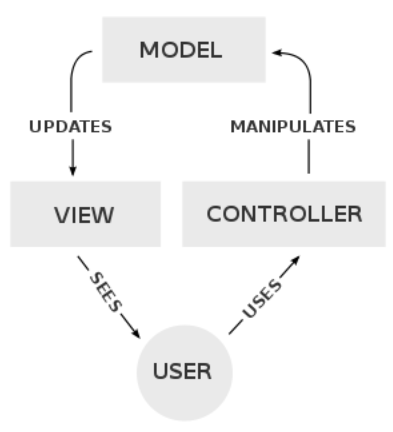
\includegraphics[scale=0.5]{img/mvc.png}
  \caption{MVC - Pattern}
  \label{fig:mapping}
\end{figure}

\begin{itemize}
  \setlength{\itemsep}{1pt}
  \setlength{\parskip}{0pt}
  \setlength{\parsep}{0pt}
  
  \item Model: enthält die zur Verfügung gestellten Daten
  \item View: ändert die Präsentation anhand von Änderungen im Model
  \item Controller: Manipuliert das Model und die View 
\end{itemize}


\subsection{Eintrittspunkt}
\label{subsec:eintrittspunkt}

Als Eintrittspunkt zur Anwendung wird eine Datei index.html definiert. Diese implementiert require.js zur Einbindung aller Javascript-Dateien und index.css zur Einbindung aller Stylesheets. \\
Für die Konfiguration von require.js wird die Datei main.js definiert, welche für das Mapping von Dateipfaden zu Namespaces zuständig ist. Die Namespaces können dann mittels asynchroner Moduldefinition dort initialisiert werden wo sie gerade gebraucht werden. Mittels requireJS werden sämtliche APIs und auch die spezifischen Anwendungsdateien initialisiert.

\subsection{Model}
\label{subsec:model}



\subsection{View}
\label{subsec:view}



\subsection{Controller}
\label{subsec:controller}









